\chapter{Weight and Balance}
\thispagestyle{fancy}
\minitoc[n] % Creating an actual minitoc

\section{Introduction}
This section describes the procedure for establishing the basic empty weight and moment of the airplane.  

It should be noted that specific information regarding the weight, arm, moment and installed equipment list for this airplane can only be found in the appropriate weight and balance records.

\section{Airplane weighing procedures}
The airplane should be weighed in the empty condition and in a level attitude.  Scales should be placed simultaneously under both main wheels and the tail wheel as shown in Figure~\ref{fig:wandb}.
\begin{figure}[h]
\centering
\includegraphics[width=1\textwidth]{wandb.eps}
\caption{Aircraft weighing orientation}
\label{fig:wandb}
\end{figure}

\subsection{Preparation}
Inflate tyres to recommended operating pressures.  Drain all fuel.  Drain all engine oil.  Move all seats to the most forward position.  Raise flaps to fully retracted position.  Place all control surfaces in neutral position.  
\subsection{Levelling}
Place scales under each wheel.  Level attitude is established at the datum line which is the cockpit rails.  
\subsection{Weighing}
With the airplane level, record the weight shown on each scale.  
\subsection{Measuring}
To keep all moments positive, a datum has been selected at a point forward of the prop spinner.  This point is 70 inches in front of the wing leading edge.  Measure the distance from both the main wheels to the aircraft datum.  Measure the distance from the tail wheel to the aircraft datum.
\subsection{Calculation}
Calculate the moment for both main wheels and the tail wheel by multiplying the distance to the datum with the measured weight for each.  Sum all the Moments and the Weights.  To obtain the empty Centre of Gravity divide the total moment by the total weight. 


\section{Weight and Balance}
The following information will enable the pilot to operate within the prescibed weight and center of gravity limitations.  

\subsection{Centre of Gravity limits}
The maximum weight and Centre of Gravity limits for both the Aerobatic and Normal Category operations are summarised in Table~\ref{tab:cofg_limits}.
\begin{table}[H]
\caption{Centre of gravity limits}
\label{tab:cofg_limits}
  \begin{tabularx}{\linewidth}{
    |>{\hsize=0.4\hsize}X| 
     >{\hsize=0.2\hsize}X|
     >{\hsize=0.2\hsize}X| 
     >{\hsize=0.2\hsize}X|
  }
%  \begin{tabular}{ |p{1in}|p{1in}|p{3.5in}| } 
 \hline
  Category & Weight \newline Maximum & C of G \newline Minimum & C of G \newline Maximum \\ 
   \hline
  Aerobatic & 1600 & 78.7" & 84.5"  \\ 
   \hline
  Normal    & 1800 & 78.7" & 86.8"  \\ 
 \hline
 \end{tabularx}
\end{table}

\subsection{Sample loading problems}
The following example in Table~\ref{tab:gross} shows the aircraft loaded to the maximum weight of 1800 lbs.  This is achieved by loading full fuel and 85lbs of the full 100 lbs baggage allowance.  A standard 170 lbs pilot and 170 lbs passenger occupy the seats.

\begin{table}[H]
\caption{Gross weight Sample loading problem}
\label{tab:gross}
  \begin{tabularx}{\linewidth}{
    |>{\hsize=0.4\hsize}X| 
     >{\hsize=0.2\hsize}X|
     >{\hsize=0.2\hsize}X| 
     >{\hsize=0.2\hsize}X| 
  }
%  \begin{tabular}{ |p{1in}|p{1in}|p{3.5in}| } 
 \hline
  Item & Weight [lbs]& Arm [inch] & Moment \newline [inch-.lbs] \\ 
 \hline
 Aircraft & 1122 & 79.14 & 88799.05 \\ 
 \hline
 Fuel (42Us Gal) & 252 & 80 & 20160.00 \\ 
 \hline
 Pilot & 170 & 97.48 & 16571.60 \\ 
 \hline
 Passenger & 170 & 97.48 & 16571.60 \\ 
 \hline
 Baggage (100 lbs max) & 85 & 126.78 & 10766.30 \\ 
 \hline
 Total (1800 lbs)& 1799 & 85.45 & 152878.55 \\ 
 \hline
\end{tabularx}
\end{table}

The second example in Table~\ref{tab:aerobatic} shows the aircraft loaded within the aerobatic limits.  The same standard 170 lbs pilot and his 170 lbs passenger can only take half tanks and little or no baggage.

\begin{table}[H]
\caption{Aerobatic weight Sample loading problem}
\label{tab:aerobatic}
  \begin{tabularx}{\linewidth}{
    |>{\hsize=0.4\hsize}X| 
     >{\hsize=0.2\hsize}X|
     >{\hsize=0.2\hsize}X| 
     >{\hsize=0.2\hsize}X| 
  }
%  \begin{tabular}{ |p{1in}|p{1in}|p{3.5in}| } 
 \hline
  Item & Weight [lbs]& Arm [inch] & Moment \newline [inch-.lbs] \\ 
 \hline
 Aircraft & 1122 & 79.14 & 88799.05 \\ 
 \hline
 Fuel (21 Us Gal) & 126 & 80 & 10080.00 \\ 
 \hline
 Pilot & 170 & 97.48 & 16571.60 \\ 
 \hline
 Passenger & 170 & 97.48 & 16571.60 \\ 
 \hline
 Baggage (100 lbs) & --- & 126.78 & --- \\ 
 \hline
 Total (1800 lbs)& 1588 & 83.14 & 132022.25 \\ 
 \hline
\end{tabularx}
\end{table}

Figure ~\ref{fig:coglimits} shows the centre of gravity limits plotted graphically.  The Normal category operation envelope is plotted with a solid blue line.  The Aerobatic operation envelope is plotted with a dashed blue line.  The gross weight sample is plotted as a solid dot and the aerobatic weight sample is plotted as a plus sign.

\begin{figure}[H]
\centering
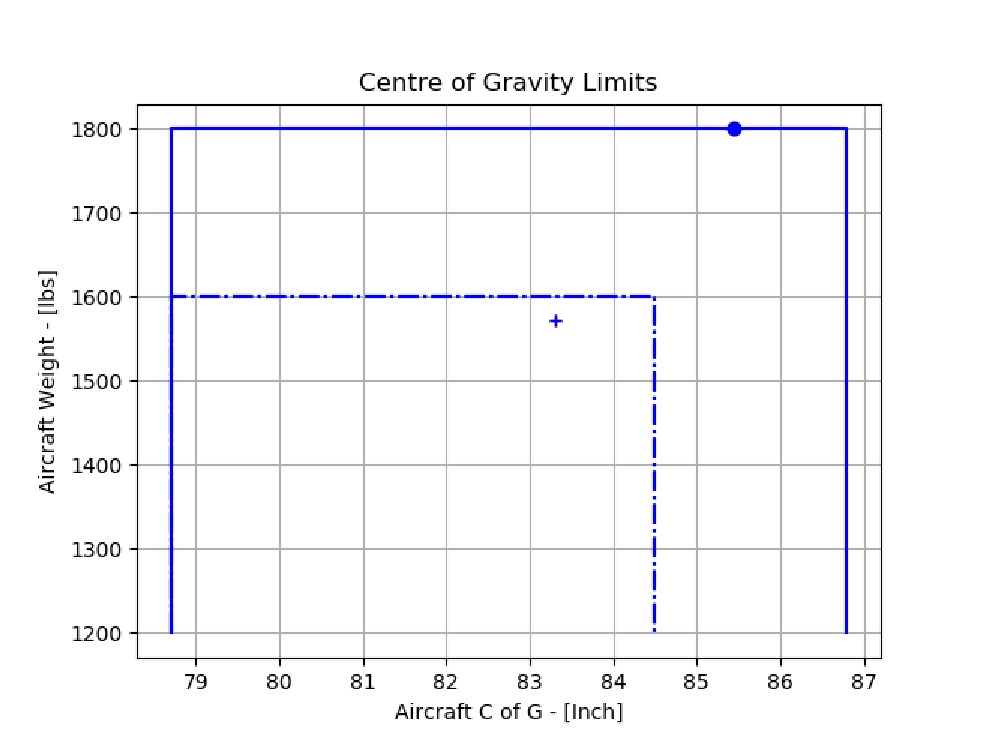
\includegraphics[width=1\textwidth]{coglimits.eps}
\caption{Aircraft weighing orientation}
\label{fig:coglimits}
\end{figure}

A blank table is provided in Table~\ref{tab:worksheet} to calculate the specific weight and balance for your aircraft.

\begin{table}[H]
\caption{Weight and Balance worksheet}
\label{tab:worksheet}
  \begin{tabularx}{\linewidth}{
    |>{\hsize=0.4\hsize}X| 
     >{\hsize=0.2\hsize}X|
     >{\hsize=0.2\hsize}X| 
     >{\hsize=0.2\hsize}X| 
  }
 \hline
  Item & Weight [lbs]& Arm [inch] & Moment \newline [inch-.lbs] \\ 
 \hline
 Aircraft & 1122 & 79.14 & 88799.05 \\ 
 \hline
 Fuel (42Us Gal) & ... & 80 &... \\ 
 \hline
 Pilot & ... & 97.48 &... \\ 
 \hline
 Passenger & ... & 97.48 &... \\ 
 \hline
 Baggage (100 lbs) & ... & 126.78 &... \\ 
 \hline
 Total (1800 lbs)& ... & ...&... \\ 
 \hline
\end{tabularx}
\end{table}

